\documentclass[11pt,aspectratio=169]{beamer}
\usepackage{amsmath,array,booktabs,graphicx,tikz}
\usetikzlibrary{arrows.meta,positioning,calc}
\input{theme_setup.tex}
\input{common_macros.tex}
\input{beamer_setup.tex}
% JJ analysis-group presentation metadata.
\newcommand{\analysisreporter}{Lekai Yao}
\newcommand{\analysisdate}{29 August 2026}

\setbeamerfont{author}{size=\small}
\setbeamerfont{institute}{size=\footnotesize}

\title[Data-driven SPS/DPS]{Data-driven SPS/DPS separation in \texorpdfstring{\Jpsi}{J/psi}-pair production}
\author[Lekai Yao]{%
  Hongbo Liao\textsuperscript{1}, Jinfeng Liu\textsuperscript{2},
  Kai Yi\textsuperscript{3}, \underline{\analysisreporter}\textsuperscript{2},
  Muhammad Ahmad\textsuperscript{2,4},\\
  Ruobing Tu\textsuperscript{1}, Shiyang Chen\textsuperscript{2},
  Shunliang Zhang\textsuperscript{2}, Taozhe Yu\textsuperscript{1},
  and Zhen Hu\textsuperscript{2}\\[0.35em]
  \analysisdate%
}
\institute[JJ collaboration]{%
  \textsuperscript{1}IHEP
  \quad \textsuperscript{2}Tsinghua University
  \quad \textsuperscript{3}Nanjing Normal University\\
  \textsuperscript{4}Texas A\&M University%
}
\date[29 August 2026]{%
  
\includegraphics[height=1.15cm]{figures/logos/CERN.png}\hspace{0.32cm}%
  
\includegraphics[height=1.15cm]{figures/logos/CMS.png}\hspace{0.32cm}%
  
\includegraphics[height=1.15cm]{figures/logos/IHEP.png}\hspace{0.32cm}%
  
\includegraphics[height=1.15cm]{figures/logos/NNU.png}\hspace{0.32cm}%
  
\includegraphics[height=1.15cm]{figures/logos/TexasAM.png}\hspace{0.32cm}%
  
\includegraphics[height=1.15cm]{figures/logos/THU.png}%
}


% Optional fast single-frame build, for example:
%   bash fastcompile_frame.sh p01
\ifdefined\onlyframes
  \expandafter\includeonlyframes\expandafter{\onlyframes}
\fi

\tikzset{
  flow/.style={draw=positive,fill=positive!8,rounded corners,thick,align=center,
    minimum height=1.05cm,text width=2.55cm,font=\small},
  dataflow/.style={draw=emphasis,fill=emphasis!8,rounded corners,thick,align=center,
    minimum height=1.05cm,text width=2.55cm,font=\small},
  arrow/.style={-{Latex[length=2.2mm]},thick,draw=neutral}
}
\newcommand{\hfig}{slides/figures/accepted/H015}
\newcommand{\hfinal}{slides/figures/accepted/H016}

\tikzset{
  bootstep/.style={draw=positive,fill=positive!8,rounded corners,thick,
    align=center,minimum height=1.25cm,text width=2.05cm,font=\small},
  bootarrow/.style={-{Latex[length=2.2mm]},thick,draw=neutral}
}

\begin{document}

\begin{frame}[plain,label=p01]
  \titlepage
\end{frame}

\begin{frame}[label=p02]{AN template fit: separating SPS and DPS shapes}
  \centering
  \small MC samples provide normalized SPS and DPS shapes in two discriminating observables.

  \begin{columns}[T,onlytextwidth]
    \column{0.49\textwidth}
      \centering
      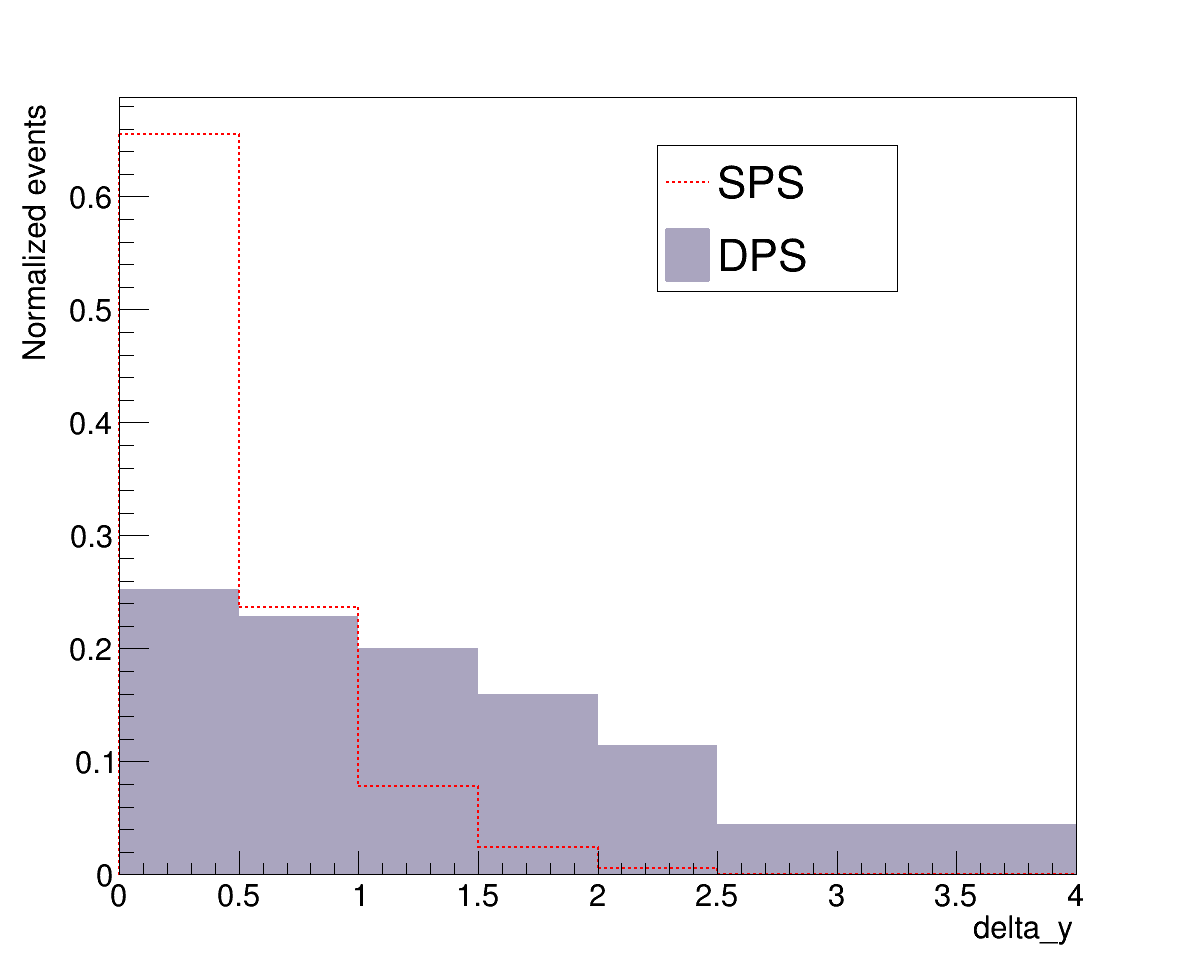
\includegraphics[height=3.50cm,keepaspectratio]{figures/an_template_fit/T_delta_y.png}\\[-0.2em]
      \textbf{$|\Delta y(\Jpsi,\Jpsi)|$:} DPS extends to larger separation
    \column{0.49\textwidth}
      \centering
      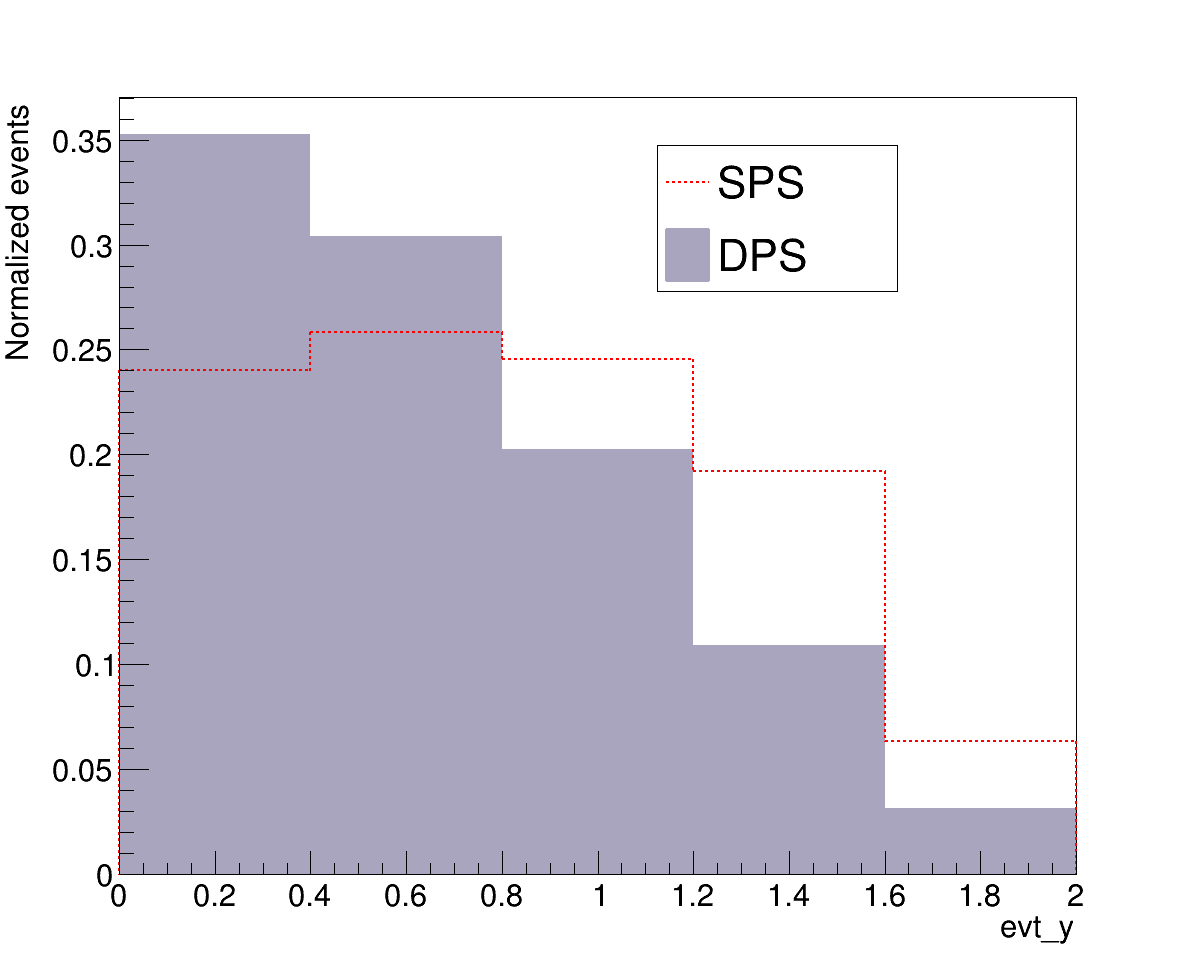
\includegraphics[height=3.50cm,keepaspectratio]{figures/an_template_fit/T_evt_y.png}\\[-0.2em]
      \textbf{$|y(\Jpsi\Jpsi)|$:} complementary SPS/DPS shape information
  \end{columns}

  \vspace{0.15em}
  \begin{block}{One shared DPS fraction in the simultaneous fit}
    \centering
    $\displaystyle p_i^{\rm fit}
      =(1-f_{\rm DPS})\,T_i^{\rm SPS}
      +f_{\rm DPS}\,T_i^{\rm DPS}$
  \end{block}
\end{frame}

\begin{frame}[label=p03]{AN simultaneous template-fit result}
  \centering
  \small The same $f_{\rm DPS}$ is fitted to both differential cross sections.

  \begin{columns}[T,onlytextwidth]
    \column{0.49\textwidth}
      \centering
      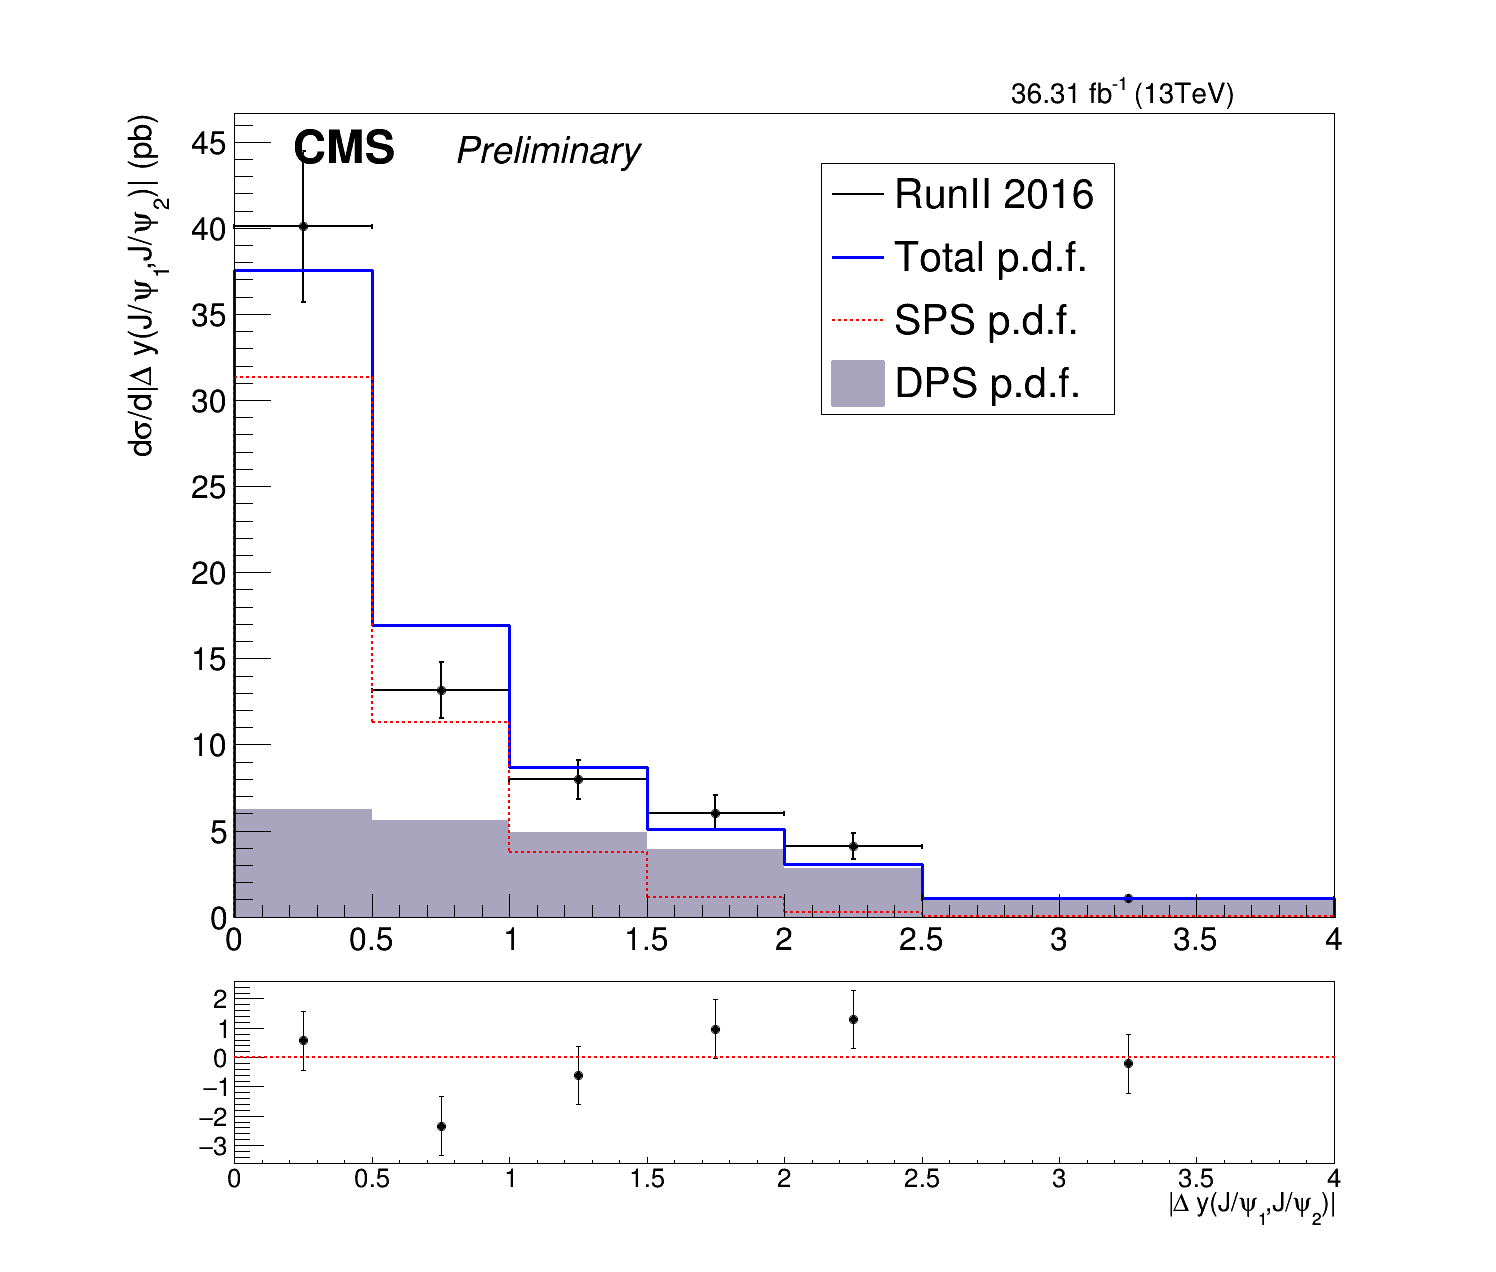
\includegraphics[height=3.90cm,keepaspectratio]{figures/an_template_fit/Template_delta_y_simul_2.png}\\[-0.1em]
      \textbf{$\mathrm d\sigma/\mathrm d|\Delta y|$}
    \column{0.49\textwidth}
      \centering
      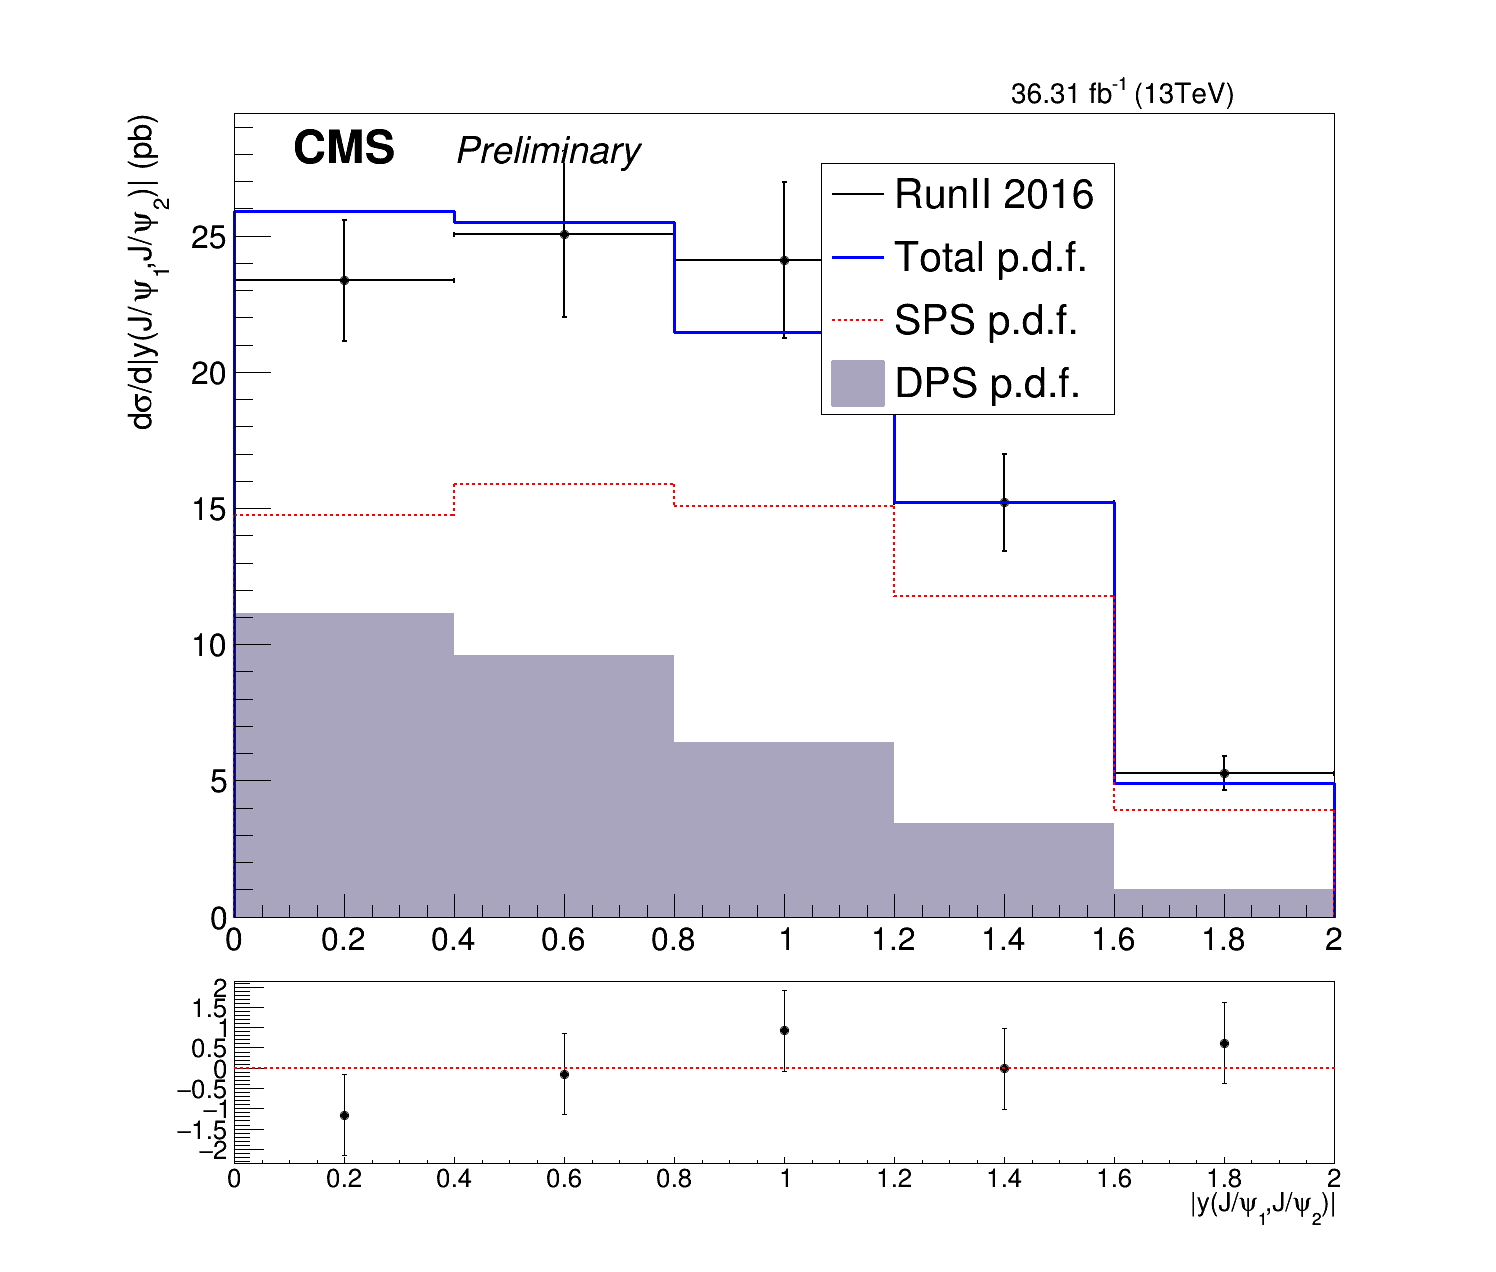
\includegraphics[height=3.90cm,keepaspectratio]{figures/an_template_fit/Template_evt_y_simul_2.png}\\[-0.1em]
      \textbf{$\mathrm d\sigma/\mathrm d|y(\Jpsi\Jpsi)|$}
  \end{columns}

  \vspace{0.1em}
  \begin{exampleblock}{Extracted DPS fraction}
    \centering
    $\displaystyle f_{\rm DPS}=0.34\pm0.10\;\text{(stat.)}
      {}^{+0.02}_{-0.17}\;\text{(syst.)}$\par
    \smallskip
    \small Systematic uncertainty from individual--simultaneous fit differences
  \end{exampleblock}
\end{frame}

\begin{frame}[label=p04]{Why pursue a data-driven separation?}
  \centering
  \small The two approaches separate the same SPS/DPS components with different inputs.

  \vspace{0.5em}
  \begin{tabular}{>{\raggedright\arraybackslash}p{0.18\textwidth}
                  >{\raggedright\arraybackslash}p{0.34\textwidth}
                  >{\raggedright\arraybackslash}p{0.38\textwidth}}
    \toprule
    & MC template fit & Data-driven separation \\
    \midrule
    Primary input & Simulated SPS and DPS shapes & Observed single-\Jpsi and pair data \\
    Main limitation & \textbf{Generator dependence}, especially the SPS shape & Mixing, factorization and control-region choices \\
    Main advantage & Fits measured differential cross sections directly & Builds templates from data kinematics and occupancy \\
    \bottomrule
  \end{tabular}

  \vfill
  \HL{\textbf{Goal: test the SPS/DPS separation with substantially different inputs and assumptions.}}
\end{frame}


\begin{frame}[label=p05]{Data-driven workflow: from source events to SPS/DPS}
  \centering
  \begin{columns}[T,onlytextwidth]
    \column{0.48\textwidth}
      \centering\textbf{Shape information}\\
      \small prompt-weighted single-\Jpsi event mixing
    \column{0.48\textwidth}
      \centering\textbf{Normalization information}\\
      \small fitted prompt-prompt yields in pair data
  \end{columns}

  \vspace{0.8em}
  \begin{tikzpicture}[node distance=0.65cm and 0.75cm]
    \node[flow] (source) {2492 selected\\source events};
    \node[flow,right=of source] (single) {Prompt weights\\for each \Jpsi slot};
    \node[flow,right=of single] (mix) {Cross-event\\mixed DPS shape};

    \node[dataflow,below=1.15cm of mix] (split) {CR normalization\\$\mathrm{PP}=\mathrm{SPS}+\mathrm{DPS}$};
    \node[dataflow,left=0.75cm of split] (pair) {Pair data\\12-cell PP yields};

    \draw[arrow] (source) -- (single);
    \draw[arrow] (single) -- (mix);
    \draw[arrow] (pair.east) -- (split.west);
    \draw[arrow] (mix.south) -- (split.north);
  \end{tikzpicture}

  \vfill
  \small ``Each \Jpsi slot'' means independent single-\Jpsi fits for \Jpsi$_1$ and \Jpsi$_2$.

  \vfill
  \HL{\textbf{The separation is built from two data constraints with different roles.}}
\end{frame}

\begin{frame}[label=p06]{Single-\Jpsi source: isolate prompt candidates before mixing}
  \centering
  \small Fit the two \Jpsi slots separately; no transverse-momentum ordering is assumed.

  \vspace{0.4em}
  \begin{tikzpicture}[node distance=0.6cm]
    \node[flow,text width=3.15cm] (model) {Unweighted 2D fit\\mass $\times$ decay length\\\muted{prompt, nonprompt, combinatorial}};
    \node[flow,text width=3.05cm,right=of model] (calib) {Stage 1: calibration\\float yields and\\resolution scales};
    \node[flow,text width=3.05cm,right=of calib] (yield) {Stage 2: yield fit\\freeze fitted scales\\compute prompt sWeights};
    \draw[arrow] (model) -- (calib);
    \draw[arrow] (calib) -- (yield);
  \end{tikzpicture}

  \vspace{0.5em}
  \begin{center}
  \begin{tabular}{lrrr}
    \toprule
    Slot & Fit entries & Prompt yield & $\sum w_{\rm prompt}$ \\
    \midrule
    $\Jpsi_1$ & 2473 & 716.92 & 716.92 \\
    $\Jpsi_2$ & 2474 & 728.72 & 728.72 \\
    \bottomrule
  \end{tabular}
  \end{center}

  \vfill
  \begin{columns}[T,onlytextwidth]
    \column{0.48\textwidth}
      \pos{\textbf{Fit acceptance}}\\[-0.1em]
      \small status $=0$, covQual $\geq2$, EDM $<0.01$
    \column{0.48\textwidth}
      \con{\textbf{Signed prompt sWeights are retained}}
  \end{columns}
\end{frame}

\begin{frame}[label=p07]{Prompt single-\Jpsi extraction in data}
  \centering
  \includegraphics[width=0.95\textwidth,height=0.79\textheight,keepaspectratio,
    trim=0 0 0 28,clip]{\hfig/single_jpsi_fit_summary.pdf}

  \vfill
  \HL{\textbf{The two \Jpsi slots are fitted independently; prompt sWeights feed event mixing.}}
\end{frame}

\begin{frame}[label=p08]{Deterministic cross-slot all-pairs mixing}
  \centering
  \small Build every allowed $\Jpsi_1(A)\otimes\Jpsi_2(B)$ pair with source events $A\neq B$.

  \vspace{0.4em}
  \begin{tikzpicture}[node distance=0.55cm]
    \node[flow,text width=2.7cm] (cart) {$2473\times2474$\\6,118,202 Cartesian pairs};
    \node[flow,text width=2.4cm,right=of cart] (same) {Reject same source\\2,456 pairs};
    \node[flow,text width=2.4cm,right=of same] (mass) {Require $m(\Jpsi\Jpsi)\geq7.5$ GeV\\53,997 rejected};
    \node[dataflow,text width=2.25cm,right=of mass] (accept) {Accepted mixed pairs\\\textbf{6,061,749}};
    \draw[arrow] (cart) -- (same);
    \draw[arrow] (same) -- (mass);
    \draw[arrow] (mass) -- (accept);
  \end{tikzpicture}

  \vspace{0.55em}
  \begin{block}{Pair weight}
    \centering
    $\displaystyle w_{AB}=w^{\rm prompt}_{1,A}\,w^{\rm prompt}_{2,B}\,C_{\rm pair}$
  \end{block}

  \begin{columns}[T,onlytextwidth]
    \column{0.48\textwidth}
      \begin{itemize}
        \item all pairs; no random sampling or mixing seed
        \item same source identified before pairing
        \item add the two \Jpsi four-vectors; require $m(\Jpsi\Jpsi)\geq7.5$ GeV
      \end{itemize}
    \column{0.48\textwidth}
      \begin{itemize}
        \item positive and negative weighted pairs retained
        \item then apply $C_{\rm pair}$: acceptance/efficiency weight
      \end{itemize}
  \end{columns}

  \vfill
  \con{\textbf{Method assumption: candidates from different source events represent independent scatters.}}
\end{frame}

\begin{frame}[label=p09]{Prompt--prompt yields in the common phase space}
  \centering
  \small A four-dimensional pair fit provides $N_{\rm PP}^{i}$ in each
  $(|\Delta y|,|\Delta\phi|)$ cell.

  \vspace{0.25em}
  \includegraphics[width=0.88\textwidth,height=0.72\textheight,keepaspectratio,
    trim=0 0 0 35,clip]{\hfig/pp_yield_map_current12.pdf}

  \vfill
  \HL{\textbf{All 12 cell fits are accepted; the fitted uncertainty is shown in every cell.}}
\end{frame}

\begin{frame}[label=p10]{The control region fixes the DPS normalization}
  \begin{columns}[T,onlytextwidth]
    \column{0.54\textwidth}
      \centering
      \includegraphics[width=\textwidth,height=0.70\textheight,keepaspectratio,
        trim=0 0 0 38,clip]{\hfig/control_region_geometry_current12.pdf}

    \column{0.43\textwidth}
      \small
      \textbf{Normalize the mixed template}
      \[
        \begin{aligned}
          \alpha &= \frac{N_{\rm PP}^{\rm CR}}{N_{\rm mix}^{\rm CR}}, \\
          N_{\rm DPS}^{i} &= \alpha N_{\rm mix}^{i}
        \end{aligned}
      \]

      \textbf{Yield definitions}\par\smallskip
      $N_{\rm PP}^{\rm CR}$: fitted prompt--prompt yield in the CR\par
      $N_{\rm mix}^{\rm CR}$, $N_{\rm mix}^{i}$: mixed-event yield in the CR / cell $i$\par
      $N_{\rm DPS}^{i}$: normalized DPS estimate in cell $i$

      \begin{alertblock}{Normalization assumption}
        Highlighted cell treated as DPS-only; SPS leakage set to zero.
      \end{alertblock}
  \end{columns}

  \vfill
  \con{CR equality is imposed by normalization; it is not a purity measurement.}
\end{frame}

\begin{frame}[label=p11]{Cell-by-cell SPS/DPS decomposition}
  \centering
  \includegraphics[width=0.95\textwidth,height=0.55\textheight,keepaspectratio,
    trim=38 92 38 88,clip]
    {\hfig/dps_sps_decomposition_current12.pdf}

  \vspace{0.15em}
  \begin{columns}[c,onlytextwidth]
    \column{0.48\textwidth}
      \centering
      $N_{\rm SPS}^{i}=N_{\rm PP}^{i}-N_{\rm DPS}^{i}$

      \smallskip
      \small Signed residuals are retained; no cell is clipped.

    \column{0.48\textwidth}
      \begin{exampleblock}{Integrated DPS fraction}
        \centering
        $\displaystyle f_{\rm DPS}=\frac{832.86}{4887.01}
          =\HL{\mathbf{0.17042}}$
      \end{exampleblock}
  \end{columns}
\end{frame}

\begin{frame}[label=p12]{Full source-event bootstrap reruns the complete estimator}
  \centering
  \small The resampling unit is the selected source event, not an individual mixed pair.

  \vspace{0.9em}
  \begin{tikzpicture}[node distance=0.32cm]
    \node[bootstep] (sample) {Resample 2492\\source events\\with\\replacement\\\muted{keep both slots paired}};
    \node[bootstep,right=of sample] (single) {Single-\Jpsi\\2 calibrations\\2 yield sPlots};
    \node[bootstep,right=of single] (mix) {All-cross-event\\mixing\\signed pair weights};
    \node[bootstep,right=of mix] (pair) {Prompt--prompt\\12 cell fits};
    \node[bootstep,right=of pair] (fdps) {CR\\normalization and $f_{\rm DPS}$ estimator};
    \draw[bootarrow] (sample) -- (single);
    \draw[bootarrow] (single) -- (mix);
    \draw[bootarrow] (mix) -- (pair);
    \draw[bootarrow] (pair) -- (fdps);
  \end{tikzpicture}

  \vspace{1.0em}
  \begin{block}{One bootstrap replica}
    \centering
    One resampled source dataset $\longrightarrow$ one complete $f_{\rm DPS}$ extraction
  \end{block}

  \vfill
  \HL{\textbf{The replica spread propagates fluctuations and correlations through the full chain.}}
\end{frame}

\begin{frame}[label=p13]{Bootstrap ensemble gives the statistical uncertainty}
  \centering
  \includegraphics[width=0.90\textwidth,height=0.64\textheight,keepaspectratio,
    trim=0 0 0 42,clip]{\hfig/bootstrap_fdps_fixed500.pdf}

  \vfill
  \begin{columns}[c,onlytextwidth]
    \column{0.47\textwidth}
      \centering
      \textbf{Fixed ensemble:} 500/500 successful replicas

    \column{0.49\textwidth}
      \begin{exampleblock}{Statistical uncertainty}
        \centering
        $\displaystyle \sigma_{\rm stat}(f_{\rm DPS})
          =\operatorname{SD}(f_{\rm DPS}^{(b)})
          =\HL{\mathbf{0.05933}}$
      \end{exampleblock}
  \end{columns}
\end{frame}

\begin{frame}[label=p14]{Single-\Jpsi category dependence}
  \begin{columns}[T,onlytextwidth]
    \begin{column}{0.56\textwidth}
      \centering
      \includegraphics[width=\textwidth,height=0.71\textheight,keepaspectratio,
        trim=0 0 0 55,clip]{\hfig/single_jpsi_category_dependence.pdf}
    \end{column}
    \begin{column}{0.41\textwidth}
      \footnotesize
      \textbf{Category refits}
      \begin{itemize}\setlength{\itemsep}{2pt}
        \item Split each \Jpsi slot independently at
          $p_{\mathrm{T}}=15\,\mathrm{GeV}$ or $|y|=1.2$.
        \item In every category, repeat the two-stage mass--$c\tau$ fit:
          calibrate resolutions, then freeze them for the yield-only sPlot.
        \item Rebuild the mixed DPS template and repeat the full extraction.
      \end{itemize}

      \textbf{Why this variation?}\par
      It probes whether kinematic dependence in the single-\Jpsi fit and prompt
      weights changes the mixed-template shape.

      \begin{exampleblock}{Category envelope}
        \centering
        $\displaystyle \Delta f_{\rm DPS}^{\rm category}
          ={}^{+0.00078}_{-0.00625}$
      \end{exampleblock}
    \end{column}
  \end{columns}
\end{frame}

\begin{frame}[label=p15]{Control-region choices set the largest envelope}
  \begin{columns}[T,onlytextwidth]
    \begin{column}{0.56\textwidth}
      \centering
      \includegraphics[width=\textwidth,height=0.71\textheight,keepaspectratio,
        trim=0 0 0 55,clip]{\hfig/control_region_variations.pdf}
    \end{column}
    \begin{column}{0.41\textwidth}
      \footnotesize
      \textbf{CR variations}
      \begin{itemize}\setlength{\itemsep}{2pt}
        \item Change $|\Delta\phi|\leq90^\circ$ to $70^\circ$ or $110^\circ$;
          alternatively raise $|\Delta y|\geq1.8$ to 2.4.
        \item Refit the PP yields in the new 2D cells, then renormalize the
          mixed template.
      \end{itemize}

      \textbf{SPS-leakage treatment}
      \begin{itemize}\setlength{\itemsep}{2pt}
        \item \emph{Zero leakage}: assign the full PP yield in the CR to DPS.
        \item \emph{MC leakage}: estimate $r_{\rm SPS}^{\rm CR}$ from SPS MC
          and subtract its contribution before setting the DPS normalization.
      \end{itemize}

      \begin{exampleblock}{Envelope over all variants}
        \centering
        $\displaystyle \Delta f_{\rm DPS}^{\rm CR}
          ={}^{+0.00783}_{-0.00649}$
      \end{exampleblock}
    \end{column}
  \end{columns}
\end{frame}

\begin{frame}[label=p16]{Pure-DPS closure probes the complete workflow}
  \begin{columns}[T,onlytextwidth]
    \begin{column}{0.56\textwidth}
      \centering
      \includegraphics[width=\textwidth,height=0.71\textheight,keepaspectratio,
        trim=0 0 0 42,clip]{\hfig/pure_dps_full_workflow_closure.pdf}
    \end{column}
    \begin{column}{0.41\textwidth}
      \footnotesize
      \textbf{Where does the sample come from?}\par
      A dedicated DPS MC sample supplies same-event \Jpsi-pair pseudo-data.
      It is \emph{not} an event-mixed sample.

      \textbf{What is tested?}
      \begin{itemize}\setlength{\itemsep}{2pt}
        \item Extract the two single-\Jpsi inputs from DPS MC.
        \item Construct the DPS template by the same cross-event mixing.
        \item Repeat the 12-cell PP fits, CR normalization and decomposition.
      \end{itemize}

      For pure DPS, $f_{\rm DPS}^{\rm exp}=1$; the workflow recovers 1.0379.

      \begin{exampleblock}{Map the closure bias to Data}
        \centering
        $0.0379\times0.1704=\HL{\mathbf{0.00645}}$
        \par\scriptsize symmetric uncertainty
      \end{exampleblock}
    \end{column}
  \end{columns}
\end{frame}

\begin{frame}[label=p17]{Three method sources combine asymmetrically}
  \centering
  \small Use each group envelope once; combine upward and downward components separately.

  \includegraphics[width=0.94\textwidth,height=0.67\textheight,keepaspectratio,
    trim=0 0 0 42,clip]{\hfig/method_systematic_breakdown.pdf}

  \vfill
    \centering
    $\displaystyle
      \sigma_{\pm}=\sqrt{\sum_g\left(\Delta_g^{\pm}\right)^2},
      \quad
      \Delta f_{\rm DPS}^{\rm method}
      =\HL{\mathbf{{}^{+0.01018}_{-0.01108}}}$
\end{frame}


% H016-F01: accepted current fraction and method-systematic groups.
\begin{frame}[label=p18]{Final data-driven DPS fraction}
  \centering
  \small The full extraction combines the fixed bootstrap ensemble with three method groups.

  \vspace{0.15em}
  \begin{columns}[T,onlytextwidth]
    \column{0.49\textwidth}
    \column{0.49\textwidth}
      \centering
      \small Three method-systematic groups\\[-0.1em]
      Separate quadrature: $+0.0102/-0.0111$
  \end{columns}

  \includegraphics[width=0.97\textwidth,height=0.62\textheight,keepaspectratio,
    trim=0 0 0 78,clip]{\hfinal/fdps_current_result.pdf}

  \vfill
  \HL{\textbf{The statistical uncertainty dominates the current $f_{\rm DPS}$ precision.}}
\end{frame}

% H016-F02: accepted preliminary sigma_DPS propagation.
\begin{frame}[label=p19]{DPS cross section from the data-driven fraction}
  \centering
  \begin{tikzpicture}
    \node[inner sep=0] (resultplot) {\includegraphics[width=0.98\textwidth,height=0.80\textheight,
      keepaspectratio,trim=0 0 0 32,clip]{\hfinal/sigma_dps_preliminary_breakdown.png}};
    \fill[white] ([xshift=1.6cm,yshift=0.45cm]resultplot.south west)
      rectangle ([xshift=5.1cm,yshift=1.30cm]resultplot.south west);
  \end{tikzpicture}

\end{frame}

% H016-F03: accepted preliminary sigma_eff propagation.
\begin{frame}[label=p20]{Effective DPS cross section}
  \centering
  \begin{tikzpicture}
    \node[inner sep=0] (resultplot) {\includegraphics[width=0.98\textwidth,height=0.80\textheight,
      keepaspectratio,trim=0 0 0 32,clip]{\hfinal/sigma_eff_preliminary_breakdown.png}};
    \fill[white] ([xshift=1.6cm,yshift=0.45cm]resultplot.south west)
      rectangle ([xshift=5.1cm,yshift= 1.65cm]resultplot.south west);
  \end{tikzpicture}

  \vfill
  \small The common branching fraction cancels; the pair-mass correction matches the single-$\Jpsi$ phase space.
\end{frame}

\begin{frame}[label=p21]{Two separations with complementary inputs}
  \centering
  \small Both methods target the SPS/DPS composition, with different shape information and uncertainty models.

  \vspace{0.45em}
  \renewcommand{\arraystretch}{1.24}
  \begin{tabular}{>{\raggedright\arraybackslash}p{0.17\textwidth}
                  >{\raggedright\arraybackslash}p{0.36\textwidth}
                  >{\raggedright\arraybackslash}p{0.36\textwidth}}
    \toprule
    & AN template fit & Data-driven separation \\
    \midrule
    Shape input & SPS/DPS simulation templates & Prompt single-$\Jpsi$ data and event mixing \\
    Normalization & Simultaneous differential-cross-section fit & Prompt-prompt yields and control region \\
    $f_{\rm DPS}$
      & $0.34\pm0.10\,{}^{+0.02}_{-0.17}$
      & $0.170\pm0.059\,{}^{+0.010}_{-0.011}$ \\
    $\sigma_{\rm DPS}$ [pb]
      & $12.6\pm3.7\,{}^{+1.1}_{-6.4}$
      & $6.34\pm2.21\,{}^{+0.57}_{-0.60}$ \\
    $\sigma_{\rm eff}$ [mb]
      & $1.26\pm0.37\,{}^{+0.64}_{-0.11}$
      & $2.48\pm0.86\,{}^{+0.25}_{-0.22}$ \\
    \bottomrule
  \end{tabular}

  \vfill
  \muted{Uncertainties are statistical, then systematic.}
\end{frame}

\begin{frame}[label=p22]{Conclusions}
  \centering
  \small A complete data-driven SPS/DPS separation is now available for the JJ analysis.

  \vspace{1.0em}
  \begin{columns}[T,onlytextwidth]
    \column{0.30\textwidth}
      \centering
      {\color{positive}\LARGE\textbf{1}}\par\medskip
      \textbf{Data construction}\par\smallskip
      \small Prompt-weighted single-$\Jpsi$ mixing supplies the DPS shape.

    \column{0.30\textwidth}
      \centering
      {\color{emphasis}\LARGE\textbf{2}}\par\medskip
      \textbf{Full uncertainty chain}\par\smallskip
      \small Source-event bootstrap plus three method-systematic groups.

    \column{0.30\textwidth}
      \centering
      {\color{negative}\LARGE\textbf{3}}\par\medskip
      \textbf{Derived observables}\par\smallskip
      \small $\sigma_{\rm DPS}$ and $\sigma_{\rm eff}$ with source-level propagation.
  \end{columns}

  \vfill
  \begin{exampleblock}{Current precision}
    \centering
    Statistical uncertainty is the leading contribution to all three data-driven results.
  \end{exampleblock}
\end{frame}

\begin{frame}[label=p23]{\strut}
  \centering
  \vfill
  \makebox[\textwidth][c]{%
    \begin{beamercolorbox}[
      wd=0.68\textwidth,
      sep=1.2em,
      center,
      rounded=true,
      shadow=true
    ]{block body}
      {\LARGE\bfseries Thanks for listening!}\par
      \vspace{1.0em}
      {\large Reporter: \analysisreporter}\par
      \vspace{0.45em}
      {\large \analysisdate}
    \end{beamercolorbox}%
  }
  \vfill
\end{frame}

\end{document}
